\documentclass{ieeeaccess}
\usepackage{cite}
\usepackage{amsmath,amssymb,amsfonts}
\usepackage{algorithmic}
\usepackage{graphicx}
\usepackage{textcomp}
\usepackage{pdfpages}
\usepackage{url}
\usepackage[utf8]{inputenc}
\usepackage{array}
\newenvironment{human}{
    \begin{quote}
    \textbf{Human:}
}{\end{quote}}

\newenvironment{chatgpt}{
    \begin{quote}
    \textbf{LLMs:}
}{\end{quote}}

\newenvironment{Questions}{
    \begin{quote}
    \textbf{Questions:}
}{\end{quote}}

\newenvironment{Answers}{
    \begin{quote}
    \textbf{Answers:}
}{\end{quote}}
\def\BibTeX{{\rm B\kern-.05em{\sc i\kern-.025em b}\kern-.08em
    T\kern-.1667em\lower.7ex\hbox{E}\kern-.125emX}}
\begin{document}
\history{Date of publication xxxx 00, 0000, date of current version xxxx 00, 0000.}
\doi{10.1109/ACCESS.2017.DOI}

\title{ChoiceMaker: Empowering Sequential Model Optimization with Query Recommendations via Large Language Models}
\author{\uppercase{Feiran (Alex) Qin}\authorrefmark{1}}
\address[1]{Computer Science Department, North Carolina State University, Raleigh, NC 27695, USA}


\tfootnote{
    %This paragraph of the first footnote will contain support 
% information, including sponsor and financial support acknowledgment. For 
% example, ``This work was supported in part by the U.S. Department of 
% Commerce under Grant BS123456.''
}

\markboth
{Author \headeretal: Preparation of Papers for IEEE TRANSACTIONS and JOURNALS}
{Author \headeretal: Preparation of Papers for IEEE TRANSACTIONS and JOURNALS}

\corresp{
    Corresponding author: Feiran (Alex) Qin (e-mail: fqin2@ncsu.edu).
    }

\begin{abstract}
Choice is not only important in human's lifes, but also crucial to software engineering. In CSC 791 Automated Software Engineering class, we are required to implement a Sequential Model Optimizer with Root Mean Square Deviation (RMSE) to the ideal value as the evaluation metric. In this paper, we propose a novel approach that empowers Sequential Model Optimization with Query Recommendations via Large Language Models (LLMs). We first compare RMSE methods with LLMs methods, and then we evaluation the ability of LLMs in different models with different number of tokens, the scalebility of few-shots-learnings, the cost of self-host and commercial models. We find that LLMs [PlaceHolder]. Overall, our approach is able to achieve a better performance than the RMSE methods. 
\end{abstract}

\begin{keywords}
Software Engineering, Large Language Models, Sequential Model Optimization
\end{keywords}

\titlepgskip=-15pt

\maketitle

\section{Introduction}
\label{sec:introduction}
\PARstart{C}{hoice} making is one of the key concerns in software engineering. Long et al.\cite{10352439} argue that, on balance, engineers spend a third of the time in planning, coding, and testing. In software engineering, more than half of the time is allocated to choice-related tasks such as planning, analysis, and testing. Making good choices is important for software reliability. . As the scale of software engineering increases, the data and parameters available become enormous. The number of control parameters of a software package grows linearly with time. Meanwhile, human understanding of those choices only ever grows sub-linearly\cite{10.1145/2786805.2786852}. It's difficult for human beings themselves to make choices that never bad, and bad choice may lead to terrible results. 30\% of all cloud computing errors come from misconfigurations of cloud software\cite{yy}, and even more alarming, 59\% of the most severe performance bugs are caused by poor configuration-- making bad choices one of the most dangerous threats to software quality\cite{10.1145/2961111.2962602}. It turns out that automatically making decisions about choices in software is a great unsung success story. AI tools are very successful at predicting how choices affect software\cite{9734271}.

In CSC 791 Automated Software Engineering \cite{791} classes, Dr. Menzies proposed Sequential Model Optimization with Root Mean Square Deviation (RMSE) to the ideal value as the evaluation metric for decision making, however, RMSE is unaware of the real meaning of data and often mislead by a large single data.

In this work, we propose a novel approach that empowers Sequential Model Optimization with Query Recommendations via Large Language Models(LLMs). The key technical challenges we faced are: 
\begin{itemize}
  

\item \textbf{How to choose the best prompts in balance of accuracy and cost?}
In order to improve the accuracy of LLMs and obtain the desired response, there are several commonly used schemes: zero-shot prompts, few-shot prompts and finetuning. The overhead and benefits of these methods are in increasing order.The cost-effectiveness ratio is determined depends on multiple variables such as the data set, the model, and the optimization objective. We would like to find a quantitative paradigm to guide tunning for datasets of similar sizes.

\item \textbf{How to evaluate the output of LLMs without ground truth?}
Similar to the previous SMO method with RMSE of telling you "how good your options are", the output of LLMs is hard to validate, regardless of whether that’s in the dataset or even feasible. We need to find a way to evaluate the output of LLMs without ground truth. Alternatively, we want to find an experience rule to reverse adjust the prompt to improve the accuracy of LLMs.

\item \textbf{Which model to choose when considering privacy, cost, and accuracy?}
There are various open-source models, such as llama2 , as well as commercial models, such as chatgpt. There are also versions of the open-source model with different token counts, such as 8b, 13b, and 33b. Open-source models are easy to self-host, and are therefore more privacy-friendly, especially when dealing with sensitive or commercial datasets. Commercial models have a performance advantage over open source models, although the gap between them is narrowing. By evaluating the ability of different models on the selection task, we hope to reveal the performance differences between different models, and the evolutionary performance of the ability of models over time.
\end{itemize}

\begin{figure*}[ht]
    \centering
    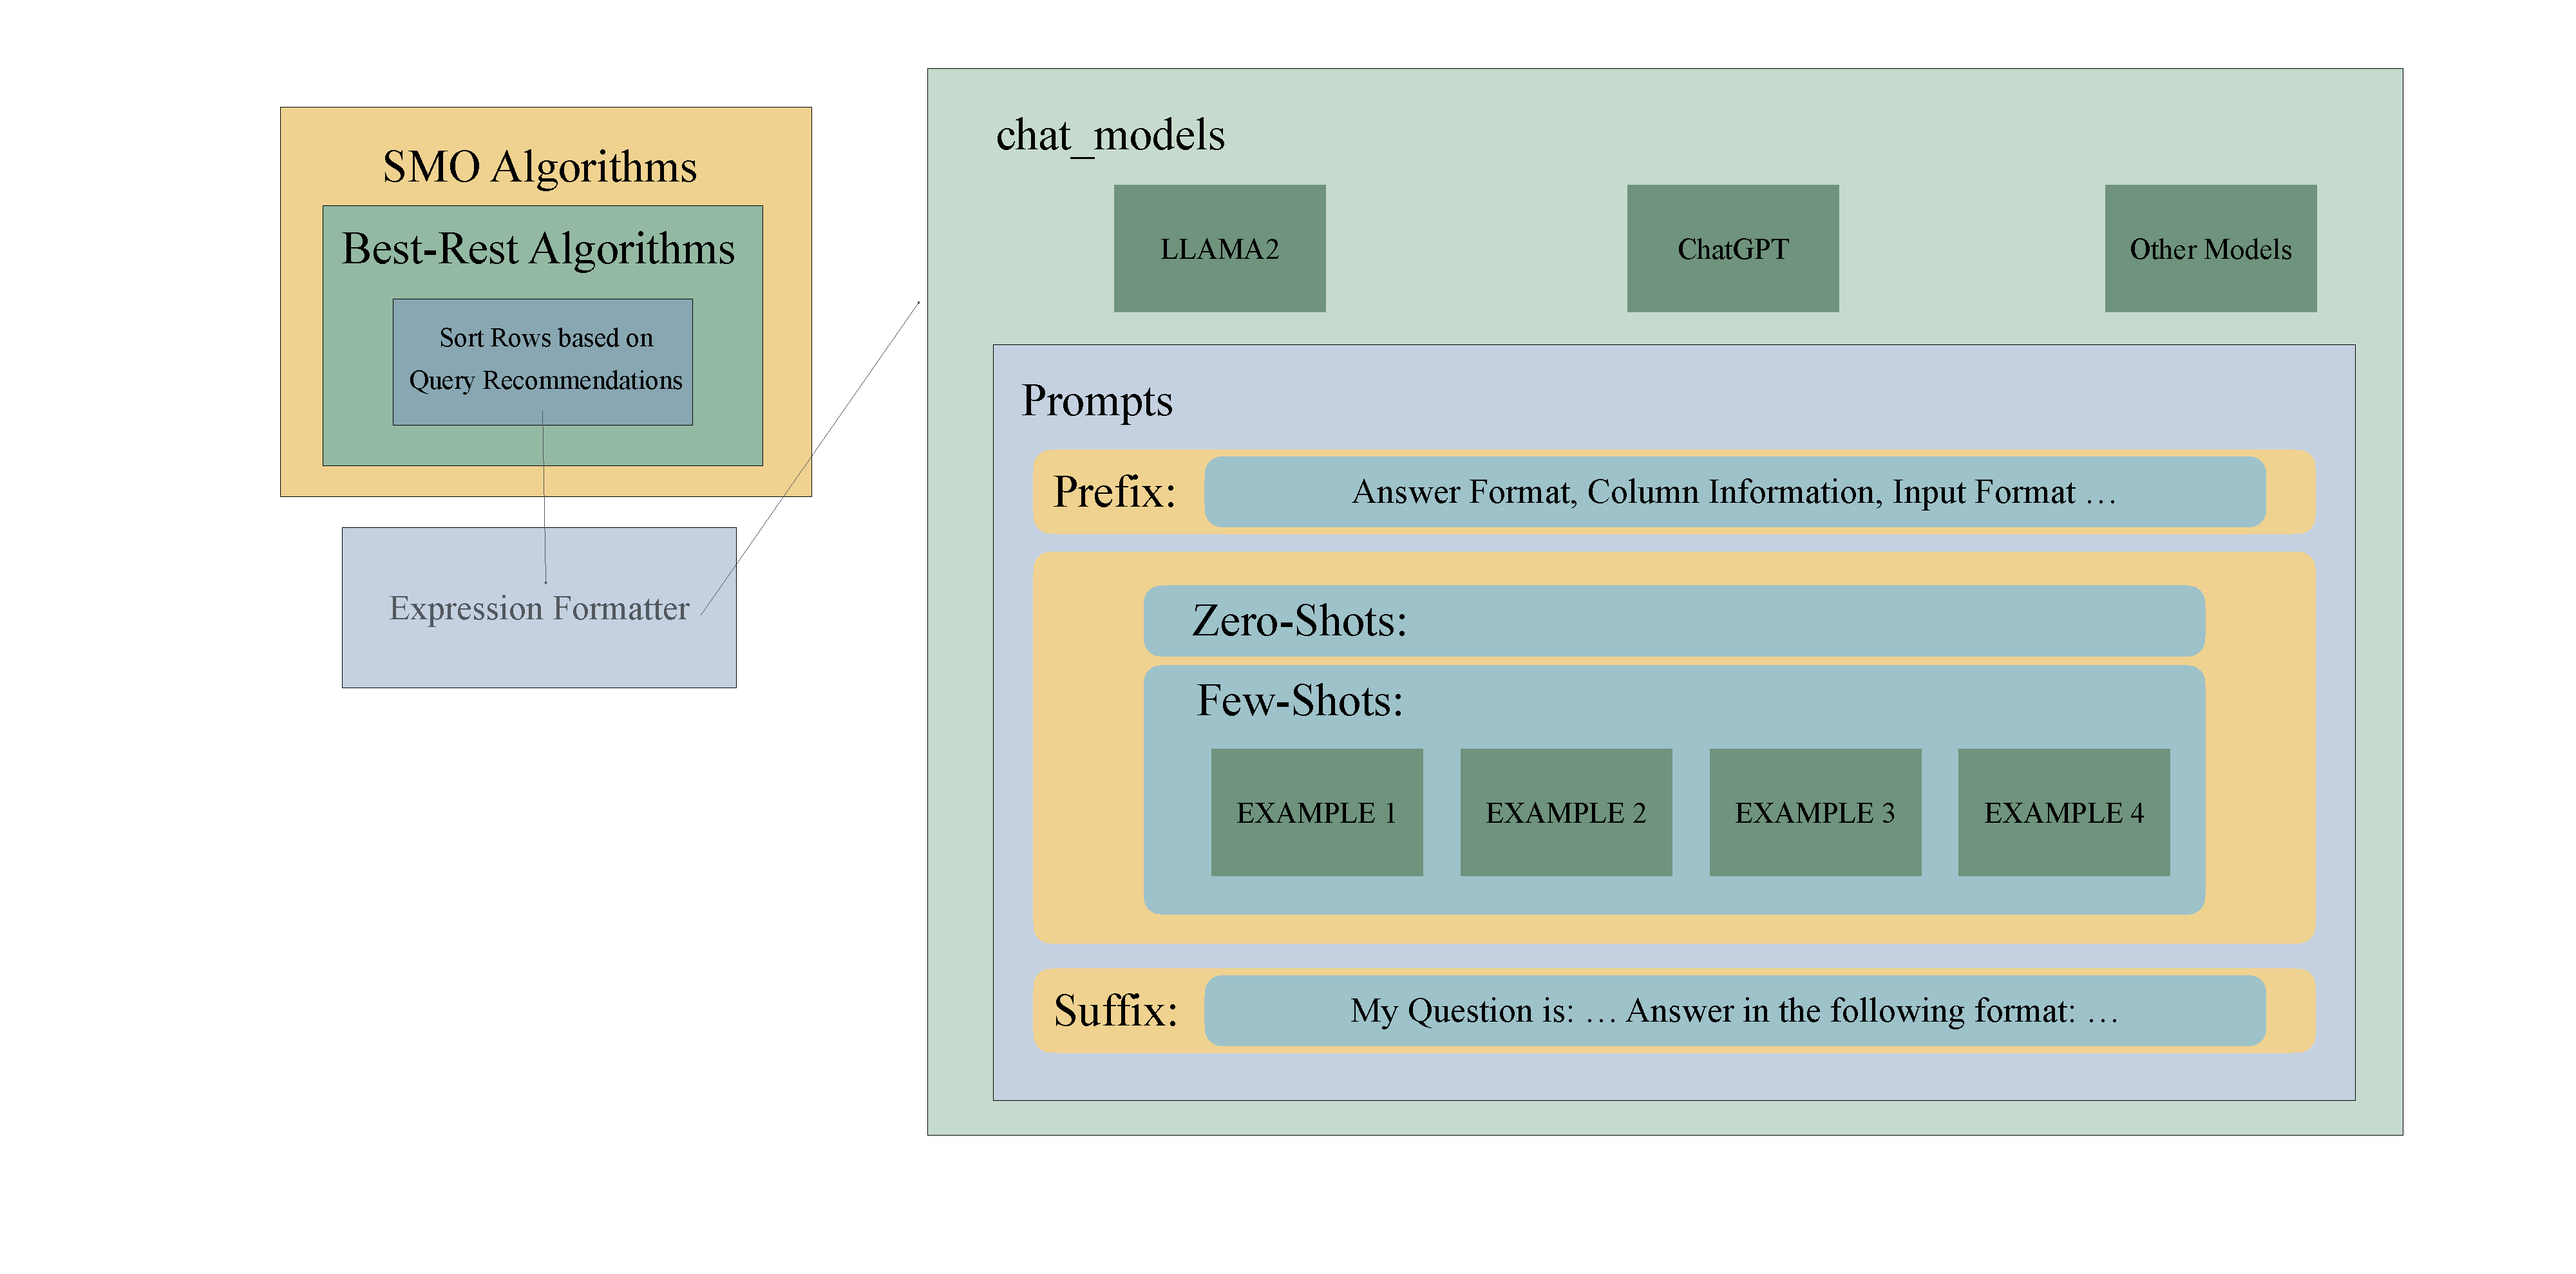
\includegraphics[page=1,width=\textwidth]{intro.pdf}
    Figure.1 An overview of ChoiceMaker \label{fig1}
  \end{figure*}

The ChoiceMaker consists of three parts, shown in Fig.\ref{fig1}: 
\begin{itemize}

\item \textbf{A modification to the SMO algorithm that sort rows based on query recommendations provided by the LLMs.}
For ease of evaluation and accuracy, we made minimal changes to the original SMO algorithm, simply replacing the original sorting algorithm with RMSE.

\item \textbf{An expression formatter}
that format the query to the LLMs specially the data rows used for sorting, and an regular expression to extract information from LLMs' outputs.

\item \textbf{A LLMs client build based on the LangChain framework.}
We introduced the LangChain library to facilitate the development of LLMs. LangChain provides an abstraction for calling APIs for different language models, and by instantiating different big predicate models, we can test different models with a unified API. The abstraction of LLMs allows us to easily switch evaluation models, such as llama2 and chatgpt. For prompts we use prefixes, examples and suffixes. In prefix, we have carefully selected the answer format, the column information and the input format for the prompt. If we want to do few-shot tunning on the model, we need to give LLMs some examples. In order to compare the performance of zero-shot with a different number of few-shots, the number of examples is optional from ${0,4,8,16}$. All examples consist of samples, and factual responses. The suffix contains the final question, usually the chosen preference, and reiterates the format of the answer to ensure that the answer can be parsed by the regular expression. In some cases of poor performance, we make artificial adjustments to the prompts, such as adding "we'll tip you" or defining the identity of the LLMs more precisely.
   
\end{itemize}

This paper makes the following contributions:
\begin{itemize}
    \item \textbf{A novel approach that empowers Sequential Model Optimization with Query Recommendations via Large Language Models(LLMs).}
    \item \textbf{Evaluation of the scalability of few shot learning}
\end{itemize}

The rest of this paper is structured as follows: Section \ref{sec:background} provides background information on the problem of choice in software engineering. Section \ref{sec:algorithms} describes the algorithms used in this work. Section \ref{sec:methods} describes the methods used in this work. Section \ref{sec:results} presents the results of the experiments. Section \ref{sec:discussion} discusses the results. Section \ref{sec:conclusion} concludes the paper.

\section{Background}
\label{sec:background}
\subsection{Sequential Model Optimization with Root Mean Square Deviation (RMSE)}
Sequential Model Optimization (SMO) is a method for optimizing the performance of a model by iteratively selecting the best model from a set of models. The RMSE is a measure of the difference between the predicted value and the actual value. The RMSE is calculated as the square root of the average of the squared differences between the predicted value and the actual value. The RMSE is a measure of the accuracy of a model, with lower values indicating better performance. The RMSE is often used as an evaluation metric in machine learning tasks, such as regression and classification. In the context of SMO, the RMSE is used to evaluate the performance of a model and select the best model from a set of models. The RMSE is calculated for each model in the set, and the model with the lowest RMSE is selected as the best model. The RMSE is used to guide the selection of models in the SMO process, with the goal of finding the model that performs best on the given task.

The RMSE formula is given by:

\begin{equation}
    \text{RMSE} = \sqrt{\frac{1}{n} \sum_{i=1}^n ( \lvert h_i - c_i \rvert)^2}
\end{equation}

where:
\begin{itemize}
    \item $n$ is the total number of observations or data points.
    \item $h_i$ represents the observed value for each data point $i$, derived from col.heaven. The "Heaven Value" (col.heaven) is a human-specific value that users can specify a \{0,1\} value to represent their preferences. For instance, if someone wants a car that's both fast and light, they could set the horsepower col.heaven to 1 and the weight col.heaven to 0 in an automotive database.
    \item $c_i$ is the calculated or expected value for each data point $i$, obtained from the expression col.norm(self.cells[col.at]). $c_i$ is a normalized value that fits within the range of 0 to 1.
    \item $(h_i - c_i)^2$ computes the square of the difference between the observed value and the calculated value for each data point.
    \item $\sqrt{\frac{1}{n} \sum_{i=1}^n (\cdot)}$ takes the square root of the average of these squared differences, yielding the RMSE, a measure of the magnitude of deviation between observed and calculated values.
\end{itemize}

The SMO algorithm is a method for optimizing the performance of a model by iteratively selecting the best model from a set of models. The SMO algorithm works as follows:

\begin{enumerate}
    \item \textbf{Shuffling:} The data rows are shuffled initially to randomize their order.
    \item \textbf{Initial Evaluation:} The method prints the root mean square deviation (d2h) for the first 6 and first 50 rows post-shuffling, providing baseline performance metrics. The choice of row count can be adjusted, noting that this depends on computational resources, Determined by variables \texttt{budget0} and \texttt{budget}.
    \item \textbf{Data Partitioning:} Rows are split into two groups, \texttt{lite} and \texttt{dark}, based on a specified budget threshold (\texttt{budget0}).
    \item \textbf{Iterative Evaluation and Selection:}
        \begin{itemize}
            \item The method iteratively processes the \texttt{lite} group by partitioning it further into \texttt{best} and \texttt{rest} segments and evaluating them.
            \item A selection process takes place where certain rows are moved from the \texttt{dark} group to the \texttt{lite} group based on evaluation results.
            \item Statistical outcomes and best-performing rows from these evaluations are recorded.
        \end{itemize}
    \item \textbf{Output:} The method returns two dictionaries, \texttt{stats} (containing mid-point evaluation data of selected rows) and \texttt{bests} (containing the best-performing rows in each iteration).
\end{enumerate}

The process of selection is based on the RMSE, which is calculated for each row in the \texttt{litSe} group. The RME is used to evaluate the performance of each row, and the best-performing rows are selected for further evaluation. The SMO algorithm iteratively selects the best-performing rows and evaluates them to find the optimal solution. The Best-Rest selection works as follows:

\begin{itemize}
    \item Initially, the function sorts the input rows based on a specific metric calculated by the \texttt{d2h} method, which presumably stands for "distance to heaven." This metric quantifies how closely each row aligns with a predefined ideal or benchmark, referred to as "heaven"
    \item \textbf{Partitioning Rows into 'best' and 'rest'}:
    The function iterates through the sorted rows and divides them into two groups. The division is based on a specified number (want).
    The first want rows (those closest to heaven) are added to the best list, implying that these rows meet or exceed a certain threshold of desirability or fit.
    The remaining rows are added to the rest list, indicating that while they are still valid, they do not match the criteria as closely as those in the best group.
\end{itemize}

\subsection{Large Language Models (LLMs)}

Large Language Models (LLMs) are a class of machine learning models that are trained on large amounts of text data. LLMs are capable of generating human-like text and have been used in a variety of natural language processing tasks, such as text generation, translation, and summarization. LLMs are typically trained on large datasets of text, such as books, articles, and websites, and are able to learn the statistical patterns in the data to generate text that is coherent and grammatically correct. LLMs are typically trained using deep learning techniques, such as neural networks, and are able to learn complex patterns in the data to generate text that is indistinguishable from human-written text. LLMs have been shown to be effective in a variety of natural language processing tasks, and have been used in a variety of applications, such as chatbots, language translation, and text summarization.

The most common LLMs are based on the transformer architecture, which was introduced by Vaswani et al. in 2017. The transformer architecture is a deep learning model that is based on self-attention mechanisms, which allow the model to focus on different parts of the input data to generate output. The transformer architecture has been shown to be effective in a variety of natural language processing tasks, and has been used in a variety of applications, such as language translation, text generation, and text summarization. The transformer architecture has been used to train large language models, such as GPT-2\cite{radford2019language}, GPT-3\cite{brown2020language}, and BERT\cite{devlin2018bert}, which have been shown to be effective in a variety of natural language processing tasks.

Popular large language models currently in use are Commercially models such as ChatGPT-4\cite{chatgpt4} and Claude-AI\cite{claudeai} and Open-source models that can be deployed by oneself like LLaMA v3\cite{llama} and Gemma\cite{gemma}.


Tawosi et al.\cite{Tawosi_2023} explores the use of search-based software engineering (SBSE) techniques to optimize the number and combination of examples provided to large language models (LLMs) for few-shot learning. This optimization aims to enhance the models' ability to estimate story points in agile software development tasks. Saparov et al.\cite{saparov2023testing} explores the ability of large language models (LLMs) to perform deductive reasoning using out-of-distribution (OOD) examples. It specifically assesses the LLMs' ability to generalize from simpler proofs to more complex ones across different dimensions: depth, width, and compositional complexity of proofs. 

New perspectives have been brought to traditional machine learning algorithms and software engineering design by LLMs. Assessing the capabilities of LLMs in these areas is still a challenge, especially with new models emerging constantly. The latest version of Llama V3 was released just days ago. Therefore, this paper hopes to replace RMSE with LLMs for providing recommendations on SMO algorithms and conduct an assessment based on that foundation. These assessments will not only evaluate the capabilities of various models but also include evaluations of few-shot learning's scalability.


\section{Algorithms}
\label{sec:algorithms}

In this section, the main discussion focuses on two key issues.
A. If we replace RMSE with a large language model and explore its potential benefits,
B. How to reasonably prompt a large language model to achieve desired outcomes.

\subsection{RMSE and LLM}
Root Mean Squared Error has limitations such as: 
\begin{itemize}
    \item RMSE is unaware of the real meaning of data and often mislead by a large single data.
    \item RMSE is a measure of the magnitude of deviation between observed and calculated values, but it is not a measure of the direction of the deviation.
    \item RMSE is a measure of the accuracy of a model, with lower values indicating better performance. However, it is not a measure of the quality of the model.
\end{itemize}
In essence, RMSE presents the deviation value of this row data, although it can reflect well in data science. However, due to a lack of understanding about the actual meaning of the data, its selection may be theoretically optimal but will not take into account whether it is feasible in real life. Another aspect to consider is that the SMO algorithm learns from the initial selection of top-performing samples. As a result, the quality of this initial selection has a significant impact on subsequent iterations and filtering processes. Therefore, the selection of the initial samples is crucial to the success of the SMO algorithm.

Therefore, this article proposes introducing large language models into the first-best rest selection to help with the choice. In previous algorithms, the "best-rest" approach would sort through data lines based on their Root Mean Squared Error (RMSE), selecting a portion of them as the "best" and relegating the remainder to be considered part of the "rest". Due to concerns about overfitting caused by small local samples, this paper considers introducing large language models to aid in sorting.

The modified Best-Rest selection algorithm works as follows:

Initially, the function sorts based on the user's preferences using a large language model. When the user provides their preference, it will be concatenated into the prompt as input for the large language model. For this large language model, we don't require it to provide a complete ranking; instead, we use "Is A better than B?" as a hint phrase and treat its response as the key for sorting.

The reason we don't use large prediction models to directly output sorted results and instead employ a combination of incremental comparison and sorting algorithms to achieve sorting effectiveness is as follows. Firstly, although SMO algorithm inputs fewer rows during one Best-Rest selection process, when dealing with larger datasets, the number of rows requiring sorting also increases significantly. Many models are limited by maximum input capacity; for instance, web-based ChatGPT can only handle 4,096 characters in each prompt. Moreover, excessive input data may impact decoder performance, especially given that large prediction models typically use big batch sizes and parallel processing to serve requests. Secondly, in some long-term memory-challenged models (e.g., llama2:8b), extremely large input data might affect their ability to sort effectively. We discovered this issue during our early experiments. In summary, we adopted the incremental comparison and sorting algorithm approach for the sake of algorithm universality and precision.

\subsection{Prompting LLMs}
In this section, we primarily introduce some of the issues that arise when writing prompts for large language models and make certain trade-offs in our design. This includes...

\subsubsection{Identity specification and Data information}

Firstly, we added pre-set identity information to the prompt, such as for a dataset of cars, we preset that an LLM's identity is that of an exceptional car sales consultant. We believe this can enhance relevance and personalization. Secondly, we found that providing detailed column information to LLMs is extremely crucial. Here are some examples below (using llama2:13b model).

\begin{human}
 ... Here are some data: \\
 Clndrs,Volume,HpX,Model,origin,Lbs-,Acc+,Mpg+ \\
 8,304,193,70,1,4732,18.5,10 \\
 8,360,215,70,1,4615,14,10 \\
 which is faster? ...
\end{human}

\begin{chatgpt}
 ... the Volume model is the way to go! ...
\end{chatgpt}

\begin{human}
    [Previous Prompts] ... Number of Cylinders, Cylinder capacity, Horsepower, Model of the car, Origin of the car, Weight of the car, Acceleration, Miles per gallon ...
\end{human}

\begin{chatgpt}
    ... with its impressive 70 horsepower engine and a svelte weight of only 14 pounds ...
\end{chatgpt}
\begin{figure}[ht]
    \centering
    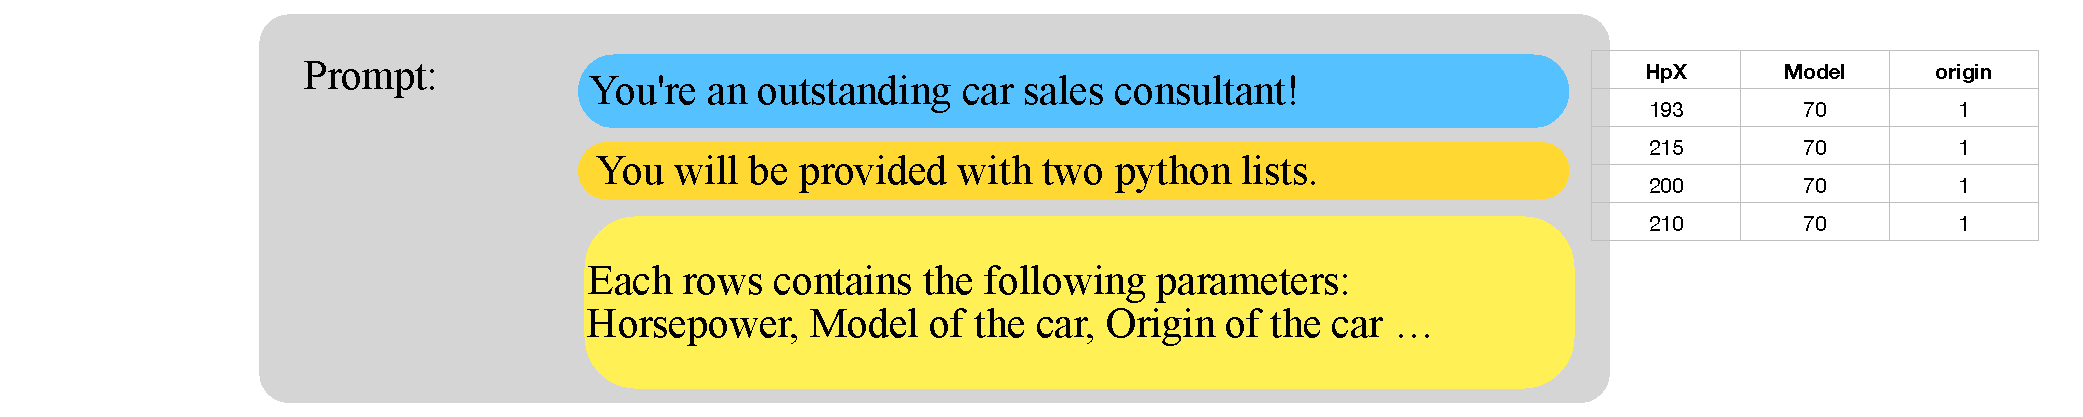
\includegraphics[page=1,width=0.5\textwidth]{llm1.pdf}
    Figure.2 Integrate identity specifications and data information into prompts \label{fig.2}
  \end{figure}
 

From this example, it's clear that if you provide more information about the data itself to LLMs, they will also consider more factors during their thought process. Despite lacking sufficient information, llama2 can still infer the meaning of all column headers. However, it appears that during its logical process, it didn't utilize all columns after all. (In reality, this depends largely on the model's capabilities; LLaMA 3 performs significantly better in this regard compared to LLaMA 2.) Therefore, as shown in Figure \ref{fig2}, identity specification and information about the data have become the prefix information of prompts.


\subsubsection{Answer Format}

We found that having LLMs respond with content formatted according to specific guidelines is a challenge, even though the \texttt{llama.cpp} library provides GBNF (GGML BNF) functionality for standardizing output. The GBNF (GGML BNF) format serves as a means of defining formal grammars to govern model outputs in \texttt{llama.cpp}. For instance, you can utilize it to compel the model to generate valid JSON or restrict its responses solely to emojis\cite{llamacpp}. However, this approach cannot be applied universally; particularly not for commercial models and those that don't employ the \texttt{llama.cpp} framework.

We attempted to specify a format for answers within prompts and simplify LLMs' responses as much as possible. We crafted a prompt that reads: "If the first list has [preference], you should answer 'A.' If the second list has more [preference], you should answer 'B.' If both lists have the same [preference], you should answer 'Same.'"

The challenge lies in language models not always responding according to format. So we've added constraints on format in both our suffix and prefix within the prompt, and are using capitalization to emphasize.

\subsubsection{Few-shot Learning}

Few-shot learning for Large Language Models (LLMs) involves the ability of these models to quickly adapt to new tasks or understand new types of queries with very limited examples, often provided directly in the prompt. This approach leverages the vast amounts of information these models have learned during their initial training, allowing them to generalize from only a handful of examples provided at inference time\cite{brown2020language}.

We utilize some ground-truth examples as few-shot learning prompts. These examples are selected from the dataset, for instance:

\begin{Questions}
    "Which car is has more horse power, A or B or Same? A: [4, 140, 86, 82, 1, 2790, 15.6, 30] B: [4, 91, 67, 82, 3, 1965, 15.7, 30]?"
\end{Questions}

\begin{Answers}
    "A"
\end{Answers}
\begin{Questions}
    "Which car is has more horse Cylinders, A or B or Same? A: [4, 140, 86, 82, 1, 2790, 15.6, 30] B: [4, 91, 67, 82, 3, 1965, 15.7, 30]?"
\end{Questions}

\begin{Answers}
    "Same"
\end{Answers}

We also tried using abstract concepts instead of ground truth to prompt the model, for instance asking about reliability rather than specific models or production methods. However, after comparison we found no improvement and there was still controversy over answer selection.

In essence, we employ example-based approaches for few-shot learning. This setup also facilitates subsequent evaluation to test the differences between zero-shot and \{2, 4, 8\}-shot learnings.

\section{Methods}
\label{sec:methods}
\subsection{Data}
I chose Auto93 as my primary dataset for evaluation. The "Auto MPG" dataset, often referred to as the "auto-mpg" or sometimes as "auto93" dataset, is a popular dataset used for regression analysis tasks in machine learning. It originates from the UCI Machine Learning Repository and includes data about various cars, specifically focusing on their fuel consumption\cite{auto_mpg_1993}.

The dataset includes information about cars from the 1970s and early 1980s. Key features in the dataset typically include in Table \ref{tbl.1}.


\begin{table*}[h!]
    \centering
    \begin{tabular}{|>{\raggedright\arraybackslash}p{3cm}|>{\raggedright\arraybackslash}p{9cm}|}
    \hline
    \textbf{Feature} & \textbf{Description} \\
    \hline
    MPG & The target variable, representing the fuel efficiency in miles per gallon. \\
    \hline
    Cylinders & The number of cylinders in the car's engine. \\
    \hline
    Displacement & The engine displacement, measured in cubic inches. \\
    \hline
    Horsepower & The power output of the engine, measured in horsepower. \\
    \hline
    Weight & The vehicle's weight in pounds. \\
    \hline
    Acceleration & The time (in seconds) it takes for the vehicle to accelerate from 0 to 60 mph. \\
    \hline
    Model Year & The year of the car model. \\
    \hline
    Origin & The origin of the car's manufacturer. \\
    \hline
    Car Name & The make and model of the car. \\
    \hline
    \end{tabular}
    \caption{Description of the Auto93 dataset features}
    \label{tbl.1}
    \end{table*}

To enhance the diversity of our data, we also conducted additional assessments on the Wine Quality dataset. The Wine Quality dataset consists of two datasets that are related to red and white variants of the Portuguese "Vinho Verde" wine. Below are the key features and details of this dataset, which are used to predict the quality of the wine on a scale from 0 (very bad) to 10 (excellent)\cite{cortez2009}. Key features in the dataset typically include in Table \ref{tbl.2}.

\begin{table*}[h!]
    \centering
    \begin{tabular}{|>{\raggedright\arraybackslash}p{4cm}|>{\raggedright\arraybackslash}p{8cm}|}
    \hline
    \textbf{Feature} & \textbf{Description} \\
    \hline
    Fixed acidity & Measures the amount of tartaric acid in the wine, which is crucial for the color, balance, and taste of the wine. \\
    \hline
    Volatile acidity & The amount of acetic acid in wine, which at too high of levels can lead to an unpleasant vinegar taste. \\
    \hline
    Citric acid & Found in small quantities, citric acid can add 'freshness' and flavor to wines. \\
    \hline
    Residual sugar & The amount of sugar remaining after fermentation stops, it's rare to find wines with less than 1 gram/liter and wines with greater than 45 grams/liter are considered sweet. \\
    \hline
    Chlorides & The amount of salt in the wine. \\
    \hline
    Free sulfur dioxide & The free form of SO\(_2\) exists in equilibrium between molecular SO\(_2\) (as a dissolved gas) and bisulfite ion; it prevents microbial growth and the oxidation of wine. \\
    \hline
    Total sulfur dioxide & Amount of free and bound forms of S02; in low concentrations, SO2 is mostly undetectable in wine, but at free SO2 concentrations over 50 ppm, SO2 becomes evident in the nose and taste of wine. \\
    \hline
    Density & The density of wine is close to that of water depending on the percent alcohol and sugar content. \\
    \hline
    pH & Describes how acidic or basic a wine is on a scale from 0 (very acidic) to 14 (very basic); most wines are between 3-4 on the pH scale. \\
    \hline
    Sulphates & A wine additive which can contribute to sulfur dioxide gas (S02) levels, wich acts as an antimicrobial and antioxidant. \\
    \hline
    Alcohol & The percent alcohol content of the wine. \\
    \hline
    Quality (target) & Score between 0 and 10. \\
    \hline
    \end{tabular}
    \caption{Features of the Wine Quality dataset}
    \label{tbl.2}
    \end{table*}
    
\subsection{Experiment Set up}

During evaluation, large language models are employed as shown in Table \ref{tbl.3}. We conducted multiple experiments, with the theme of evaluating the LLaMA 3:8B model. As for our experimental results and questions we want to answer, they are as follows:

\subsubsection{Comparison between SMO with RMSE and SMO with LLMs}
The primary experiment is a comparison between the differences of using SMO with and without LLMs, as well as comparing it to using SMO with only RMSE. We employed Llama 3 as our large language model to provide guidance for the SMO algorithm, and conducted evaluations on two datasets: Auto93 and Wine Quality. As before, we used RMSE as our evaluation metric; performed 20 rounds of random experiments; compared the results' RMSE values from using SMO with only RMSE versus using it with LLMs in each round's experiment result. Additionally, we also compared the average RMSE value for each filtered trial during those 20 attempts. As a default setting, we employ an 8-shot approach in few-shot learning.
\subsubsection{Comparative testing with varying numbers of few-shot instances}
We will attempt to fine-tune models using zero shot learning (no examples), one example per class for one shot learning and four examples per class for four shots. We will also explore eight shots and sixteen shots where we have eight or sixteen examples respectively. The dataset we use is Auto-93. The experimental indicators are the average Root Mean Squared Error (RMSE) of 20 random test results. We hope to explore how different quantities of few-shot learning affect accuracy.

\subsubsection{Cost-performance considerations for various large language models}

In this experiment, we will compare the cost-performance ratios of various large-scale language models. We will evaluate models of different sizes and complexities, including ChatGPT-4, LLaMA3, LLaMA2:8B, and LLaMA2:13B among others. To assess these models' performance in terms of accuracy, speed, and computational resource requirements we will use the Auto93 dataset and 8-shot-learning to evaluate them.

\subsection{Evaluation metrics}
We use Root Mean Square Error (RMSE) as our primary evaluation metric. RMSE is a standard way to measure the error of a model in predicting quantitative data. The formula for RMSE is:

\begin{equation}
    RMSE = \sqrt{\frac{1}{n}\sum_{i=1}^{n}(\lvert y_i - \hat{y}_i \rvert )^2}
\end{equation}

where $y_i$ is the actual value, $\hat{y}_i$ is the predicted value, and $n$ is the number of observations. Lower RMSE values indicate better fit.

We will conduct twenty random experiments and use the best-selected RMSE value as an evaluation metric. When comparing each other, we will display the average RMSE values of all twenty experiments for each experiment result. In cases where multiple methods are compared, we will display the overall average of all 20 experimental results' RMSE values.

\subsection{Statistical Methods}
To perform significance and effect size tests on the RMSE from two experimental methods where each method has been tested 20 times, we follow these steps:

\subsubsection*{Significance Test using t-test}
The t-test for two independent samples is given by:
\begin{equation}
    t = \frac{\overline{X}_1 - \overline{X}_2}{\sqrt{\frac{s_1^2}{n_1} + \frac{s_2^2}{n_2}}}
\end{equation}
where $\overline{X}_1$ and $\overline{X}_2$ are the means of the RMSEs for each method, $s_1^2$ and $s_2^2$ are the variances, and $n_1$ and $n_2$ are the sample sizes (both 20).

This will tell if the difference in RMSE between the two models is statistically significant.

\subsubsection*{Effect Size Test using Cohen's d}
Cohen's d for independent measures is calculated as:
\begin{equation}
    d = \frac{\overline{X}_1 - \overline{X}_2}{s_{pooled}}
\end{equation}
with the pooled standard deviation defined as:
\begin{equation}
    s_{pooled} = \sqrt{\frac{(n_1-1)s_1^2 + (n_2-1)s_2^2}{n_1 + n_2 - 2}}
\end{equation}
The resulting Cohen's d would tell the size of the effect in standardized units.
\begin{table*}[h!]
    \centering
    \begin{tabular}{|>{\raggedright\arraybackslash}p{2.5cm}|>{\raggedright\arraybackslash}p{3cm}|>{\raggedright\arraybackslash}p{4.5cm}|}
    \hline
    \textbf{Model} & \textbf{Bits} & \textbf{Description} \\
    \hline
    ChatGPT-4 & N/A & An advanced language model by OpenAI with enhanced reasoning, context awareness, and depth of knowledge. \\
    \hline
    LLaMA2 & 8-bit & Meta's efficiency-focused model offering reduced computational requirements while maintaining high language task performance. \\
    \hline
    LLaMA2 & 13-bit & Similar to the 8-bit version, but with potentially greater accuracy and computational efficiency balance. \\
    \hline
    LLaMA3 & 8-bit & The latest in the LLaMA series, optimized for language understanding and computational efficiency. \\
    \hline
    \end{tabular}
    \caption{Summary of Advanced AI Language Models}
    \label{tbl.3}
    \end{table*}

\section{Results}
\label{sec:results}
\subsubsection{Comparison between SMO with RMSE and SMO with LLMs}
\begin{figure}
    \centering
    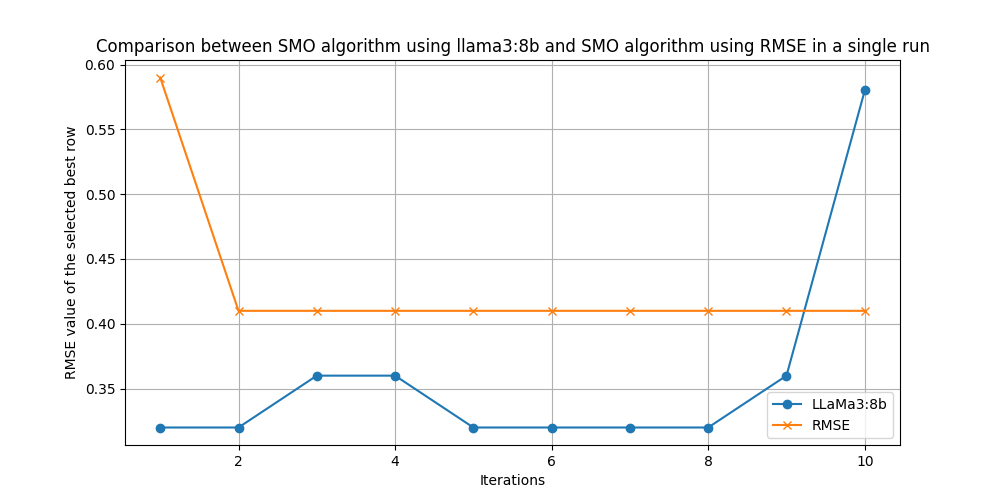
\includegraphics[page=1,width=0.5\textwidth]{llama3_8b_vs_rmse.png}
    Figure.3 Comparison between SMO with RMSE and SMO with LLMs on DataSet Auto 93 (Single Run) \label{fig.3}
  \end{figure}

\section{Discussion}
\label{sec:discussion}

\section{Conclusion}
\label{sec:conclusion}


% \appendices

% Appendixes, if needed, appear before the acknowledgment.

\section*{Acknowledgment}





\begin{thebibliography}{00}

\bibitem{10352439}Long, D., Drylie, S., Ritschel, J. \& Koschnick, C. An Assessment of Rules of Thumb for Software Phase Management, and the Relationship Between Phase Effort and Schedule Success. {\em IEEE Transactions On Software Engineering}. \textbf{50}, 209-219 (2024)

\bibitem{yy} Yuanyuan Zhou, Keynote address, IEEE Automated Software Engineering conference, San Diego, California, USA, 2019. 

\bibitem{10.1145/2786805.2786852}Xu, T., Jin, L., Fan, X., Zhou, Y., Pasupathy, S. \& Talwadker, R. Hey, you have given me too many knobs!: understanding and dealing with over-designed configuration in system software. {\em Proceedings Of The 2015 10th Joint Meeting On Foundations Of Software Engineering}. pp. 307-319 (2015), https://doi.org/10.1145/2786805.2786852

\bibitem{10.1145/2961111.2962602}Han, X. \& Yu, T. An Empirical Study on Performance Bugs for Highly Configurable Software Systems. {\em Proceedings Of The 10th ACM/IEEE International Symposium On Empirical Software Engineering And Measurement}. (2016), https://doi.org/10.1145/2961111.2962602

\bibitem{9734271}Siegmund, N., Dorn, J., Weber, M., Kaltenecker, C. \& Apel, S. Green Configuration: Can Artificial Intelligence Help Reduce Energy Consumption of Configurable Software Systems?. {\em Computer}. \textbf{55}, 74-81 (2022)

\bibitem{791} Tim Menzies. Automated Software Engineering (2024 Spring) \emph{https://github.com/txt/aa24/tree/main}. 

\bibitem{Tawosi_2023} V. Tawosi, S. Alamir, and X. Liu, 
``Search-Based Optimisation of LLM Learning Shots for Story Point Estimation,'' 
in \emph{Lecture Notes in Computer Science}, 
Springer Nature Switzerland, 2023, pp. 123-129.
\textsc{doi}: \url{10.1007/978-3-031-48796-5_9}.

\bibitem{saparov2023testing}
Abulhair Saparov, Richard Yuanzhe Pang, Vishakh Padmakumar, Nitish Joshi, Seyed Mehran Kazemi, Najoung Kim, and He He.
\textit{Testing the General Deductive Reasoning Capacity of Large Language Models Using OOD Examples},
arXiv preprint arXiv:2305.15269, 2023.


\bibitem{radford2019language}
Alec Radford, Jeffrey Wu, Rewon Child, David Luan, Dario Amodei, and Ilya Sutskever.
\textit{Language Models are Unsupervised Multitask Learners},
OpenAI Blog, 2019.
URL: \url{https://cdn.openai.com/better-language-models/language_models_are_unsupervised_multitask_learners.pdf}

\bibitem{brown2020language}
Tom B. Brown, Benjamin Mann, Nick Ryder, Melanie Subbiah, Jared Kaplan, Prafulla Dhariwal, Arvind Neelakantan, Pranav Shyam, Girish Sastry, Amanda Askell, Sandhini Agarwal, Ariel Herbert-Voss, Gretchen Krueger, Tom Henighan, Rewon Child, Aditya Ramesh, Daniel M. Ziegler, Jeffrey Wu, Clemens Winter, Christopher Hesse, Mark Chen, Eric Sigler, Mateusz Litwin, Scott Gray, Benjamin Chess, Jack Clark, Christopher Berner, Sam McCandlish, Alec Radford, Ilya Sutskever, and Dario Amodei.
\textit{Language Models are Few-Shot Learners},
arXiv preprint arXiv:2005.14165, 2020.

\bibitem{devlin2018bert}
Jacob Devlin, Ming-Wei Chang, Kenton Lee, and Kristina Toutanova.
\textit{BERT: Pre-training of Deep Bidirectional Transformers for Language Understanding},
Proceedings of the 2019 Conference of the North American Chapter of the Association for Computational Linguistics (NAACL), 2018.
arXiv preprint arXiv:1810.04805.


\bibitem{chatgpt4}
OpenAI.
\textit{Introducing ChatGPT-4},
OpenAI Blog, 2023.
URL: \url{https://openai.com/blog/chatgpt-4}

\bibitem{claudeai}
Anthropic.
\textit{Claude: A helpful, honest, and harmless AI},
Anthropic Blog, 2023.
URL: \url{https://www.anthropic.com/claude}

\bibitem{llama}
Hugo Touvron, Thibaut Lavril, Gautier Izacard, Xavier Martinet, Marie-Anne Lachaux, Timothée Lacroix, Baptiste Rozière, Naman Goyal, Eric Hambro, Faisal Azhar, Aurélien Rodriguez, Armand Joulin, Edouard Grave, and Guillaume Lample.
\textit{LLaMA: Open and efficient foundation language models},
arXiv preprint arXiv:2302.13971, 2023.

\bibitem{gemma}
Google Research.
\textit{Introducing Gemma: Google's Generative Model for Multitask Applications},
Google AI Blog, 2023.
URL: \url{https://ai.googleblog.com/2023/gemma}

\bibitem{llamacpp}
Georgi Gerganov,
\textit{README for llama.cpp grammars}.
GitHub repository,
2024.
\url{https://github.com/ggerganov/llama.cpp/blob/master/grammars/README.md}.
Accessed: April 21, 2024.

\bibitem{auto_mpg_1993}
R. Quinlan (1993). Auto MPG. UCI Machine Learning Repository. Available: \url{https://doi.org/10.24432/C5859H}

\bibitem{cortez2009}
Paulo Cortez, A. Cerdeira, F. Almeida, T. Matos, and J. Reis (2009). 
\textit{Wine Quality}. 
UCI Machine Learning Repository. 
Available: \url{https://archive.ics.uci.edu/ml/datasets/Wine+Quality}

\end{thebibliography}
% \begin{IEEEbiography}[{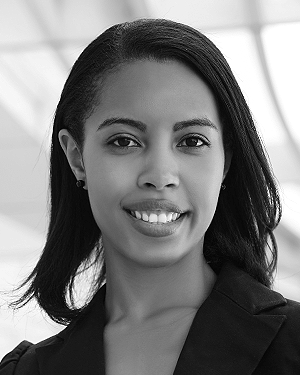
\includegraphics[width=1in,height=1.25in,clip,keepaspectratio]{a1.png}}]{First A. Author} (M'76--SM'81--F'87) and all authors may include 
% biographies. Biographies are often not included in conference-related
% papers. This author became a Member (M) of IEEE in 1976, a Senior
% Member (SM) in 1981, and a Fellow (F) in 1987. The first paragraph may
% contain a place and/or date of birth (list place, then date). Next,
% the author's educational background is listed. The degrees should be
% listed with type of degree in what field, which institution, city,
% state, and country, and year the degree was earned. The author's major
% field of study should be lower-cased. 

% The second paragraph uses the pronoun of the person (he or she) and not the 
% author's last name. It lists military and work experience, including summer 
% and fellowship jobs. Job titles are capitalized. The current job must have a 
% location; previous positions may be listed 
% without one. Information concerning previous publications may be included. 
% Try not to list more than three books or published articles. The format for 
% listing publishers of a book within the biography is: title of book 
% (publisher name, year) similar to a reference. Current and previous research 
% interests end the paragraph. The third paragraph begins with the author's 
% title and last name (e.g., Dr.\ Smith, Prof.\ Jones, Mr.\ Kajor, Ms.\ Hunter). 
% List any memberships in professional societies other than the IEEE. Finally, 
% list any awards and work for IEEE committees and publications. If a 
% photograph is provided, it should be of good quality, and 
% professional-looking. Following are two examples of an author's biography.
% \end{IEEEbiography}

% \begin{IEEEbiography}[{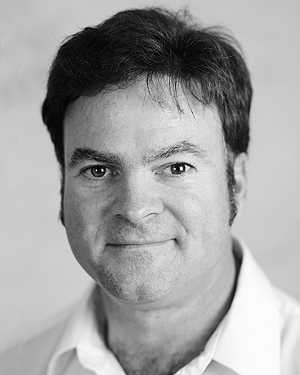
\includegraphics[width=1in,height=1.25in,clip,keepaspectratio]{a2.png}}]{Second B. Author} was born in Greenwich Village, New York, NY, USA in 
% 1977. He received the B.S. and M.S. degrees in aerospace engineering from 
% the University of Virginia, Charlottesville, in 2001 and the Ph.D. degree in 
% mechanical engineering from Drexel University, Philadelphia, PA, in 2008.

% From 2001 to 2004, he was a Research Assistant with the Princeton Plasma 
% Physics Laboratory. Since 2009, he has been an Assistant Professor with the 
% Mechanical Engineering Department, Texas A{\&}M University, College Station. 
% He is the author of three books, more than 150 articles, and more than 70 
% inventions. His research interests include high-pressure and high-density 
% nonthermal plasma discharge processes and applications, microscale plasma 
% discharges, discharges in liquids, spectroscopic diagnostics, plasma 
% propulsion, and innovation plasma applications. He is an Associate Editor of 
% the journal \emph{Earth, Moon, Planets}, and holds two patents. 

% Dr. Author was a recipient of the International Association of Geomagnetism 
% and Aeronomy Young Scientist Award for Excellence in 2008, and the IEEE 
% Electromagnetic Compatibility Society Best Symposium Paper Award in 2011. 
% \end{IEEEbiography}

% \begin{IEEEbiography}[{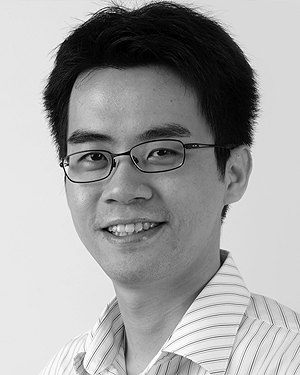
\includegraphics[width=1in,height=1.25in,clip,keepaspectratio]{a3.png}}]{Third C. Author, Jr.} (M'87) received the B.S. degree in mechanical 
% engineering from National Chung Cheng University, Chiayi, Taiwan, in 2004 
% and the M.S. degree in mechanical engineering from National Tsing Hua 
% University, Hsinchu, Taiwan, in 2006. He is currently pursuing the Ph.D. 
% degree in mechanical engineering at Texas A{\&}M University, College 
% Station, TX, USA.

% From 2008 to 2009, he was a Research Assistant with the Institute of 
% Physics, Academia Sinica, Tapei, Taiwan. His research interest includes the 
% development of surface processing and biological/medical treatment 
% techniques using nonthermal atmospheric pressure plasmas, fundamental study 
% of plasma sources, and fabrication of micro- or nanostructured surfaces. 

% Mr. Author's awards and honors include the Frew Fellowship (Australian 
% Academy of Science), the I. I. Rabi Prize (APS), the European Frequency and 
% Time Forum Award, the Carl Zeiss Research Award, the William F. Meggers 
% Award and the Adolph Lomb Medal (OSA).
% \end{IEEEbiography}

\EOD

\end{document}
